% *******************************************************************************
% * Copyright (c) 2007 by Elexis
% * All rights reserved. This document and the accompanying materials
% * are made available under the terms of the Eclipse Public License v1.0
% * which accompanies this distribution, and is available at
% * http://www.eclipse.org/legal/epl-v10.html
% *
% * Contributors:
% *    G. Weirich - initial implementation
% *
% *  $Id: laborview.tex 2819 2007-07-16 13:38:22Z rgw_ch $
% *******************************************************************************
% !Mode:: "TeX:UTF-8" (encoding info for WinEdt)

\section{Laboranzeige-View}
\index Labor!Eingabe
\index Labor!Anzeige
Bei Elexis werden sowohl interne als auch externe Laborbefunde, sowohl
automatisch eingelesene als auch manuell eigegebene Befunde in derselben Sicht
angezeigt.

Die  Anzeige eines Befundes wird bestimmt durch
\begin{itemize}
  \item Ein Laboritem, zu dem dieser Befund gehört
  \item Ein Datum, an dem dieser Befund erhoben wurde
  \item Einen Patienten, zu dem dieser Befund gehört
\end{itemize}

Das Laboritem definiert, wie und wo der Laborbefund angezeigt werden soll, und
zu welchem Typ von Laborwerten er gehört. Das Erstellen von Labritems ist in der Regel nur bei der Installation des
Programms notwendig, bzw. dann, wenn Sie neue Laborparameter in Ihre
Standardbesimmungen aufnehmen möchten. Das genaue Vorgehen ist unter Konfiguration (S. \pageref{config:labor} genauer beschrieben.

 %\usepackage{graphics} is needed for \includegraphics
\begin{figure}[htp]
\begin{center}
  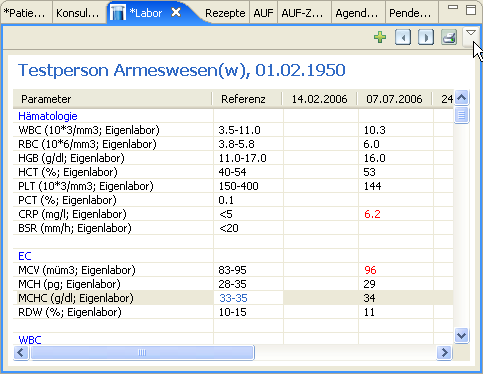
\includegraphics{images/labview}
  \caption{Labor-Anzeige}
  \label{fig:labview}
\end{center}
\end{figure}

\subsection{Manuelle Eingabe}
Um Laborwerte manuell einzutragen, gehen Sie so vor:
\begin{itemize}
    \item Wenn für das gewünschte Datum noch keine Spalte exstiert, klicken Sie auf das grüne Pluszeichen rechts oben, um ein Datum anzugeben.
    \item klicken Sie auf die Zeile und Spalte, wo Sie einen Laborwert eingeben möchten. Tippen Sie den Wert ein und verlassen Sie das Feld mit der Eingabetaste, oder der Pfeil-nach-unten-Taste.
\end{itemize} 
Wenn ein Laborparameter numerisch ist, und der eingegebene Wert ausserhalb des Referenzbereichs ist, wird der Wert in rot angezeigt. Sie können diese ANzeige auch manuell ein- und ausschalten, indem Sie den Wert mit der rechten Maustaste anklicken und das Häkchen vor "pathologisch" setzen oder löschen.

\subsection{Automatisches Einlesen}
\index{Labor:automatisches Einlesen}
Elexis kann Laborwerte selbstverständlich auch automatisch einlesen. Hierfür dient das View-Menu rechts oben:\\
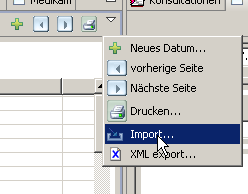
\includegraphics{images/labor6}\\
Klicken Sie auf \textit{import} und wählen Sie in der dann erscheinenden Dialogbox die Quelle für die einzulesenden Laborwerte aus. Was für Quellen hier angeboten werden, hängt von den vorhandenen Laborimport-Plugins ab. In Frage kommen Laborgeräte und verschiedene externe Labors. Eine aktuelle Liste aller vorhandenen Laborimport-Plugins finden Sie auf http://www.elexis.ch

\subsection{Laborblatt drucken}
Um ein Laborblatt auszudrucken, klciken Sie auf das Drucker-Symbol rechts oben. Dies erstellt eine Tabelle innterhalb einer Textvorlage
 